%!TeX root = ../complex_net_report_senacheribbe.tex
\graphicspath{{../assignment2/figures/}}

\subsection{Introduction}

In this assignment, we simulated different epidemic processes on a real graph. The chosen network is a small snapshot of Facebook graph, obtained from users participating in an app (\cite{db_fb}). Each node represents a person, while the edges are friendship between people.\\
In \cref{fig:2_sparsity}, the sparsity of the adjacency matrix of the graph is reported. The blocky structure indicates the presence of different communities, ie part of the graph which are closely connected together.\\
% The numbering of the nodes is sorted such that nodes from the same community have adjacent numbers, yielding to these blocks around the diagonal.
It is interesting to study epidemic processes on social networks, because they are a good model for the spread of information across people.\\ Moreover, since our graph shows this community structure, we can try to see how the information spread inside a community and from one community to another.


\begin{figure} [!ht]
	\centering
	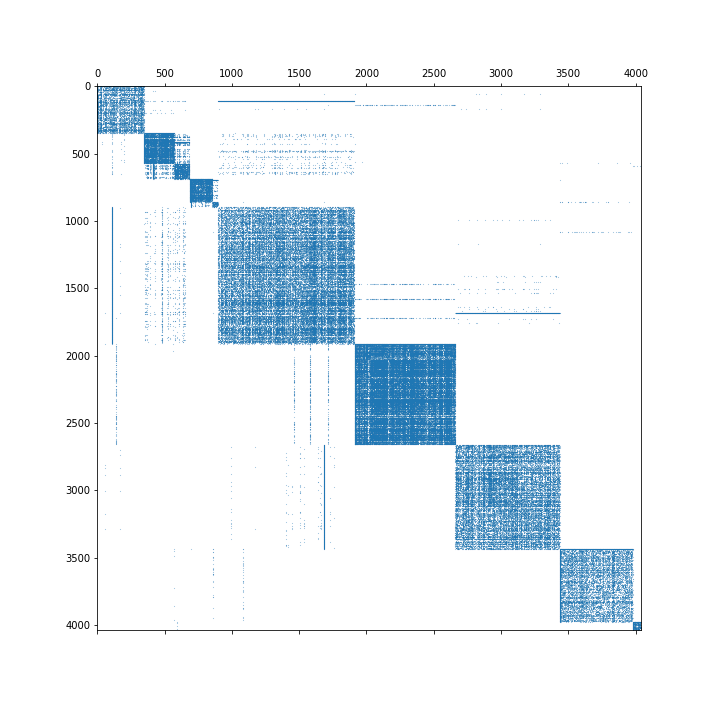
\includegraphics[width=.5\linewidth, clip, trim={2cm 2cm 2cm 2cm}]{sparsity}
	\caption{Sparsity of social network graph with  $n = 4039$ and $m = 88234$}
	\label{fig:2_sparsity}
\end{figure}


\subsection{Simple SI model}
The first model studied is a simple SI model: when a node is infected, it can infect with a probability $p$ each adjacent node. To implement this model, a FIFO queue is used to keep track of which infected node is to be processed and has to spread the infection to the neighbours. More details are reported in \cref{algo:2_simple}. The function  \textit{simple\_model} outputs:
\begin{itemize}
	\item $n\_infected$, a vector containing the number of infected nodes for each generation (generation is increased each time the infection spread to a neighbour node and it can represent the distance from the source node)
	\item $infected$, a vector that for each node associates 1 if was infected in the process, 0 otherwise. 
\end{itemize}

To test the model, we simulate an infection starting from node $\#2300$, which is in the middle of one community block.
We choose different values of $p$ (probability of spreading the infection) to test its effect on the process. Following a Monte Carlo approach, $1000$ simulations are run for each value of $p$ and the outputs are averaged. \\
The result of simulation are shown in \cref{fig:2_simple}, where we plot the fraction of infected nodes against the generations. $p=1$ is the degenerate case where all the neighbouring nodes get the infection and this is equivalent to a graph search (BFS).\\
From the graph we can notice that by increasing the generation, we have more nodes infected, since the algorithm is let run more and propagate for longer the infection. Moreover by increasing $p$, we have an higher probability to spread the infection, therefore an higher fraction of nodes gets infected.

\begin{figure} [!ht]
	\centering
	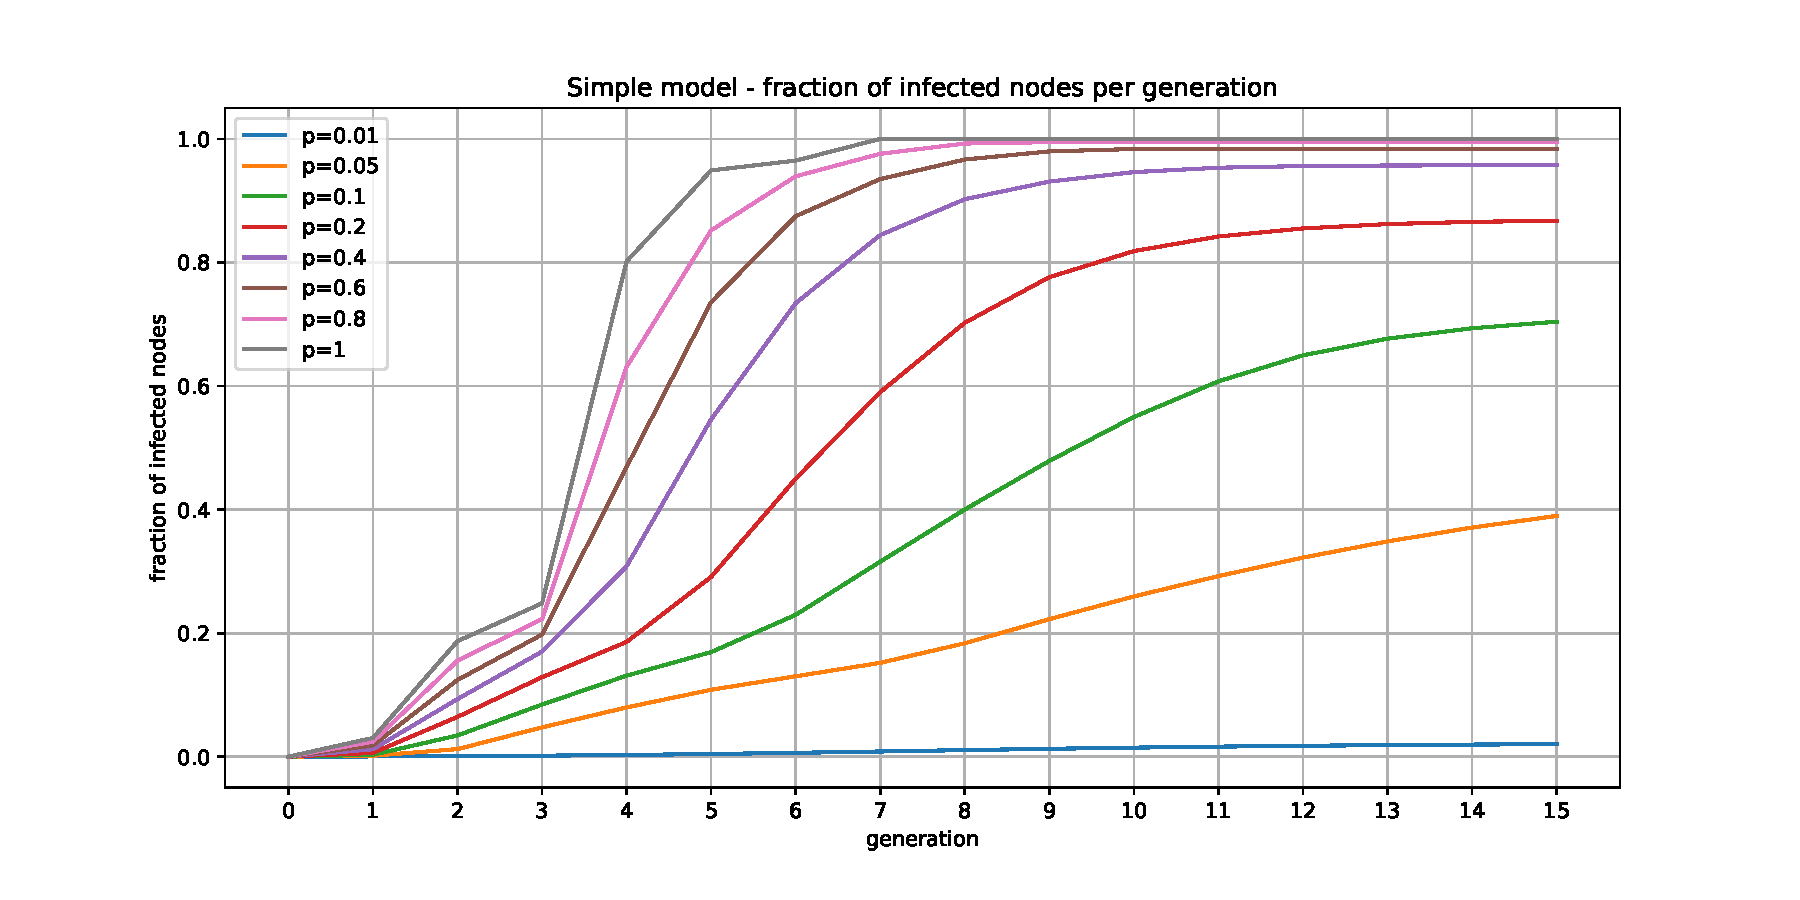
\includegraphics[width=.65\linewidth]{simple}
	\caption{Number of infected nodes per generation for the simple model algorithm}
	\label{fig:2_simple}
\end{figure}

In \cref{fig:2_probability} instead, the model has been run with $p=0.1$ for 8 generations, starting again from node $\#2300$ and averaging $1000$ simulations. The plot shows for each node the probability of it to be infected (1 means that in all $1000$ simulations it was infected, 0 if it was never infected). We can clearly notice the the information started in node $\#2300$ spreads easily in the community of the node itself and to the adjacent community of node $\#1500$ (probably because the two communities are well connected). The information struggles instead to be received from the other block communities.

\begin{figure} [!ht]
	\centering
	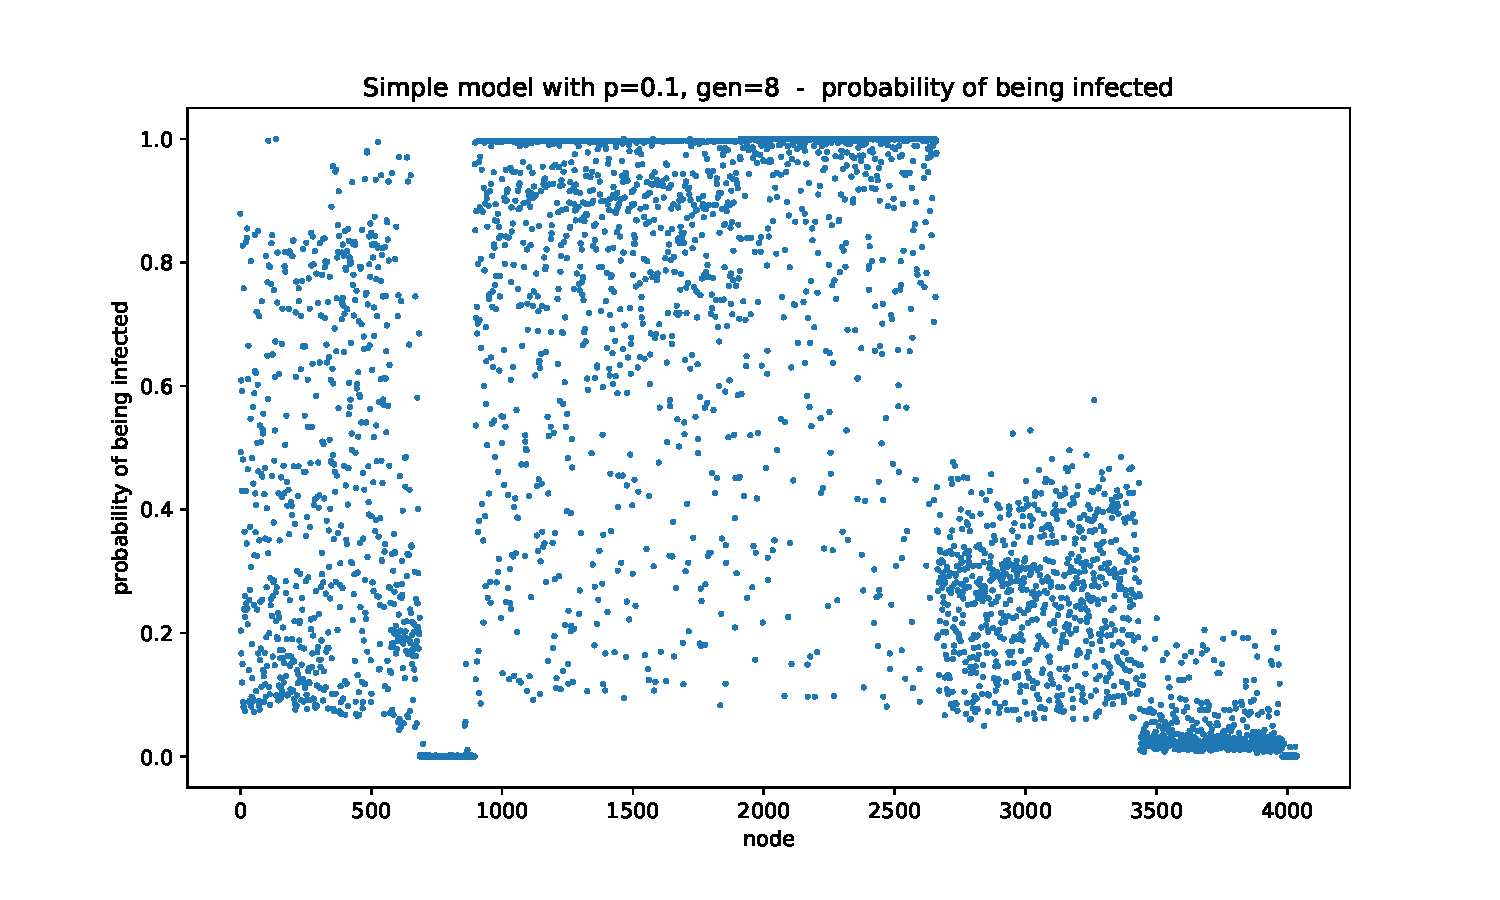
\includegraphics[width=.55\linewidth]{probability}
	\caption{Probability of being infected for the simple model algorithm}
	\label{fig:2_probability}
\end{figure}


\begin{algorithm}[!ht]
	\caption{Simple SI model}
	\label{algo:2_simple}
	\begin{algorithmic}[1]
		\Function{simple\_model}{$graph, p, max\_gen, starting$}
		
		\State $n\_infected \gets$ vector, size $max\_gen+1$, full of $0$
		\State $infected \gets$ vector, size $n$, full of $0$
		\State $queue \gets$ empty queue\\
		\Comment{$queue$ contains a tuple of 2 elements: node id and generation}
		\\
		
		\State enqueue $((starting, 0)) \to queue$
		\State $infected[starting] \gets 1$
		\State $n\_infected[0] \gets 1$	
		\\
		\While {$queue$ not empty and $g\le max\_gen$}
		\State dequeue $((v,g)) \gets queue$
		
		\For{$i \in $ neighbours of $v$}		
		\If{$infected[i]=0$ and $random()<p$} \Comment{$random() \sim Uniform[0,1]$}
		\State $infected[i] \gets 1$
		\State $n\_infected[g+1]+=1$				
		\State enqueue $((i, g+1)) \to queue$
		\EndIf
		\EndFor
		\EndWhile
		\\	
		\State \Return $cumsum(n\_infected)/n$ and $infected$
		\EndFunction
	\end{algorithmic}
\end{algorithm}

\subsection{Bootstrap percolation}\label{sec:2_boot}

As second epidemic process, we implemented the bootstrap percolation: a node gets infected if at least $r$ of its neighbours are infected. 
The pseudocode presented in \cref{algo:2_bootstrap} is very similar to \cref{algo:2_simple}, with the difference that $starting$ is now a vector of initial infected nodes and the addition of the vector $pressure$ which counts how many infected nodes are adjacent to the considered node. When the latter becomes $\ge r$ the considered node becomes infected itself and it's added in the queue.

The results of the simulations are shown in \cref{fig:2_bootstrap}, for different values of $r$. The starting points are 10 nodes inside the community of nodes from $\#2000$ to $\#2500$ (the same considered with the previous model). No Monte Carlo approach is needed, since once fixed the starting nodes, the spreading is deterministic. As we can notice from the picture, for the case $r=5$ the infection is not able to propagate, because too many adjacent nodes are required to get infected. Smaller values of $r$ makes easier to pass the infection. The case $r=1$ is a degenerate case, which is a simple graph search.

\begin{figure} [H]
	\centering
	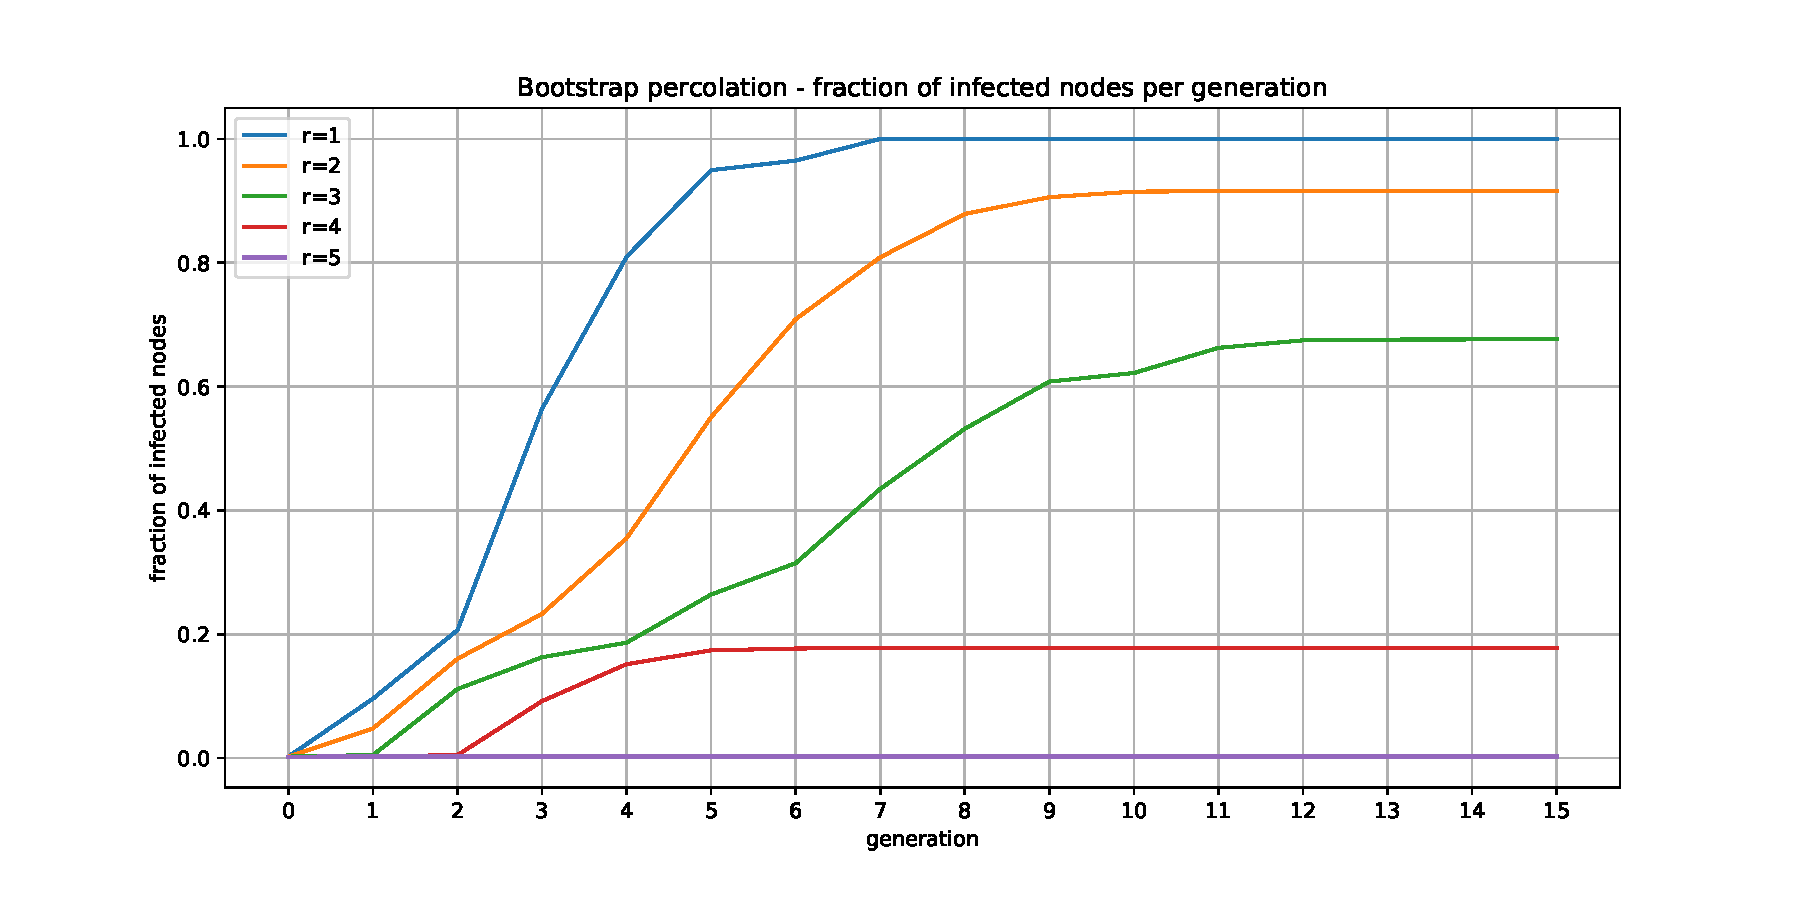
\includegraphics[width=.7\linewidth]{bootstrap}
	\caption{Number of infected nodes per generation for bootstrap percolation}
	\label{fig:2_bootstrap}
\end{figure}

\begin{algorithm}[H]
	\caption{Bootstrap percolation}
	\label{algo:2_bootstrap}
	\begin{algorithmic}[1]
		\Function{bootstrap\_percolation}{$graph, r, max\_gen, starting$}
		
		\State $n\_infected \gets$ vector, size $max\_gen+1$, full of $0$
		\State $infected \gets$ vector, size $n$, full of $0$
		\State $pressure \gets$ vector, size $n$, full of $0$
		\State $queue \gets$ empty queue\\
		\Comment{$queue$ contains a tuple of 2 elements: node id and generation}
		\\
		
		
		\State enqueue $((starting, 0)) \to queue$
		\State $infected[starting] \gets 1$
		\State $n\_infected[0] \gets length(starting)$	
		\\
		\While {$queue$ not empty and $g\le max\_gen$}
		\State dequeue $((v,g)) \gets queue$
		
		\For{$i \in $ neighbours of $v$}		
		\State $pressure[i] +=1$
		\If{$infected[i]=0$ and $pressure[i]\ge r$}
		\State $infected[i] \gets 1$
		\State $n\_infected[g+1]+=1$				
		\State enqueue $((i, g+1)) \to queue$
		\EndIf
		\EndFor
		\EndWhile
		\\	
		\State \Return $cumsum(n\_infected)/n$ and $infected$
		\EndFunction
	\end{algorithmic}
\end{algorithm}
\pagebreak

\subsection{Bootstrap percolation (stochastic version)}
Finally the bootstrap percolation presented in \cref{sec:2_boot} is modified to allow different values of $r$. Now instead of fixing it to a constant value, it is expressed as a vector that associates for each number of infected neighbours a probability to get the infection.\\ For example, the following mapping $r=[1 \to 0,\quad 2 \to 0.4,\quad 3 \to 1]$ means:
\begin{itemize}
	\item if a node has 1 infected neighbour $\rightarrow$ probability 0 of becoming infected
	\item if a node has 2 infected neighbours $\rightarrow$ probability 0.4 of becoming infected
	\item if a node has 3 or more infected neighbours $\rightarrow$ probability 1 of becoming infected
\end{itemize}
The sampling of the probability distribution is performed each time the number of adjacent infected neighbours changes. The algorithm to implement this version is exactly the same as \cref{algo:2_bootstrap}, with a small modification in the \textbf{If statement}.

Using the mapping above, we run $1000$ simulations and take the average. The starting points are the same 10 nodes between $\#2000$ and $\#2500$ considered before. The results are shown in \cref{fig:2_boot_stoc} and compared with a deterministic bootstrap with $r=2$ and $r=3$. As expected since our mapping is in the middle between $r=2$ and $r=3$ (we allow sometimes $r=2$ but always $r=3$), the curve representing the fraction of infected nodes is bounded by the two deterministic cases.

\begin{figure} [!ht]
	\centering
	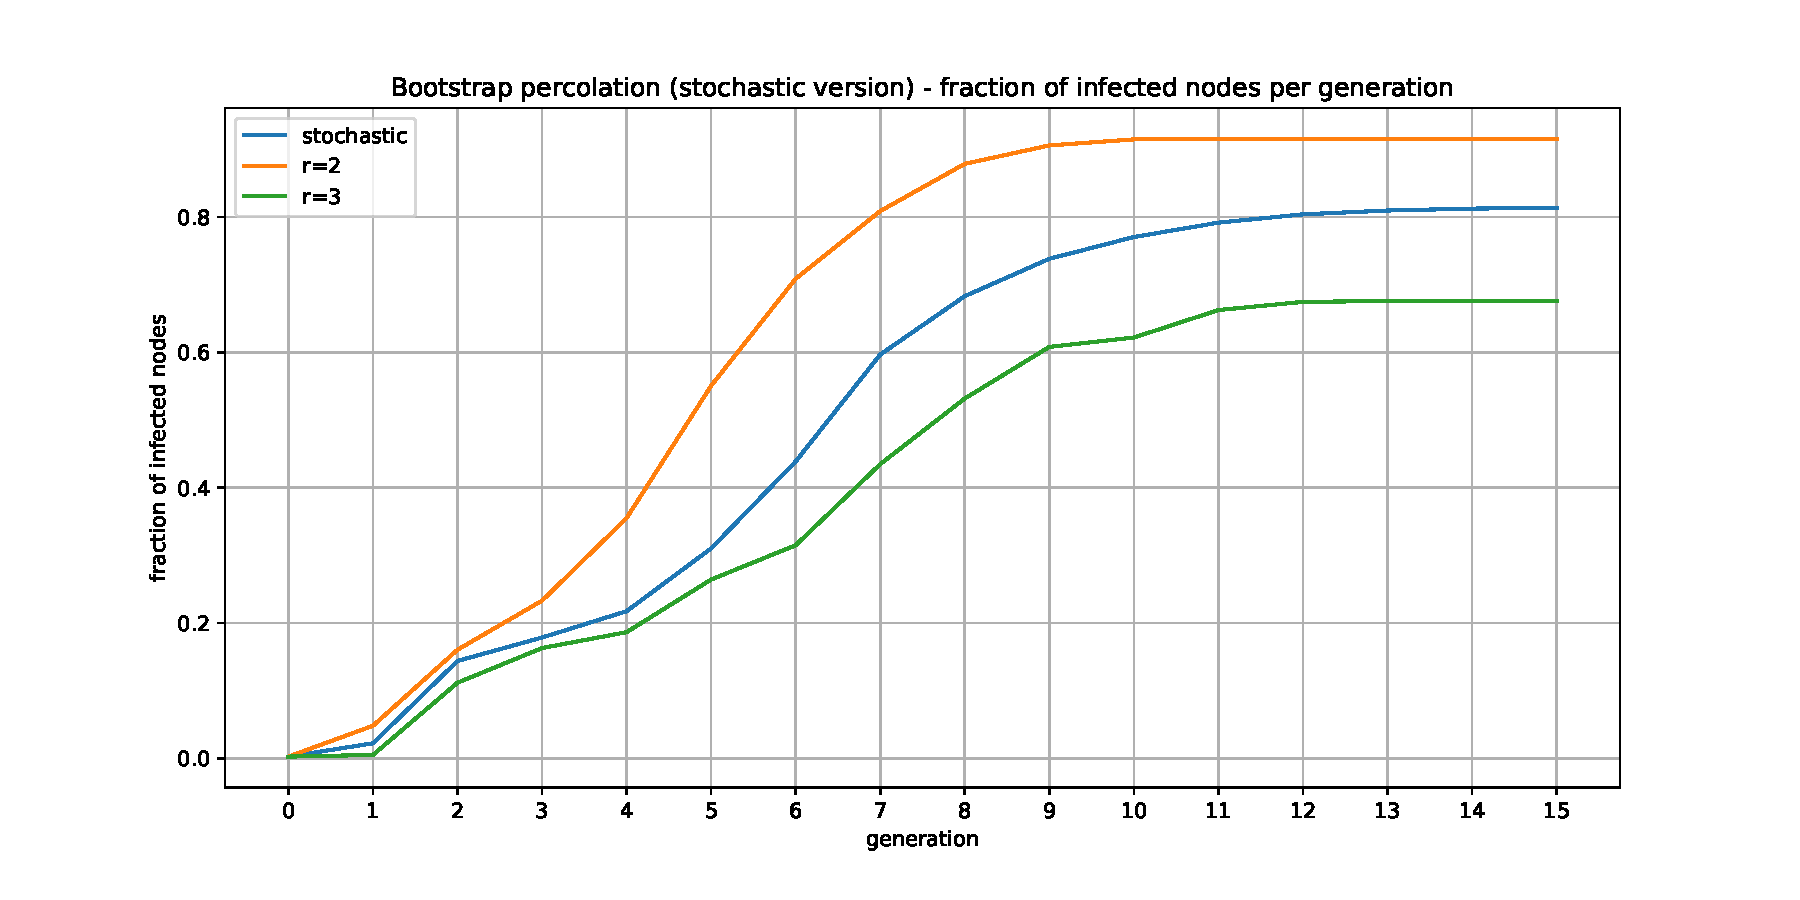
\includegraphics[width=.7\linewidth]{bootstrap_stoc}
	\caption{Number of infected nodes per generation for bootstrap percolation (stochastic version)}
	\label{fig:2_boot_stoc}
\end{figure}
